\subsection{Robotetik}
	Hvis bilerne kommer til at blive selvkørende, er der et spørgsmål som ofte bliver stillet igen og igen. I tilfælde af bilen kommer ud for et uheld, hvad skal bilen så gøre? Skal bilen gøre det samme som en person bag rettet, og forsøge at undvige faren forude og så ramme en skolebus eller en børnehave klasse ude på tur? Skal bilen handle logisk og ofre de personer i den pågældende bil? Er den logiske løsning overhovedet hvad vi mennesker rent faktisk ønsker, eller skal de selvkørende biler forsøge distribuere konsekvensen på alle parter? Enhver person bag rettet vil typisk forsøge at beskytte sig selv først og fremmest, samt deres familie, frem for andre trafikanter, så er dette hvad en selvkørende bil også skal gøre? Hvem ville sætte sig ind i en bil som vil ofre dit liv, hvis den kan redde andres?
	
	Disse er alle spørgsmål som bliver stillet når der tales robotetik, og væsentlige spørgsmål vi stadig ikke har et formelt svar på endnu.
	\begin{figure}[h!]
		\centering
		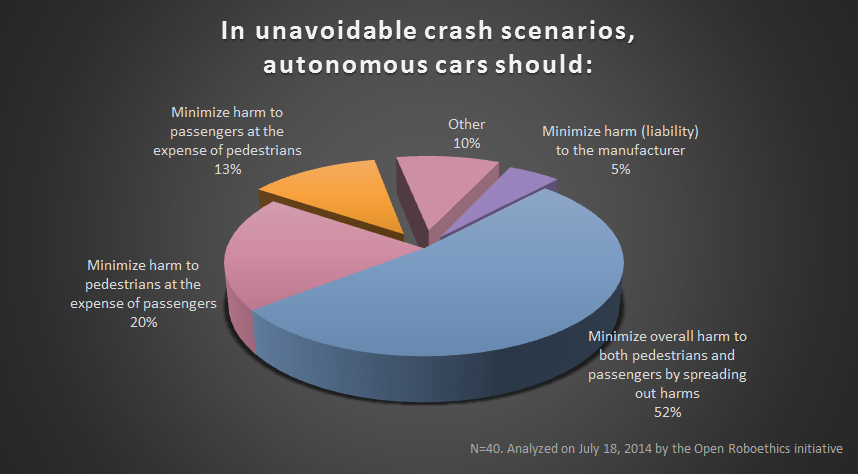
\includegraphics[width=0.8\textwidth]{images/roboethics-2.jpg}
		\caption{Undersøgelse om hvad folk vil foretrække i en uundgåelig ulykke}
		\label{fig:etik_accident}
	\end{figure}
	\cite{rob_etik}
	 I et senarie hvor et tog kommer kørende ned af en bane imod tre mennesker spændt fast til togskinnerne, men inden toget støder mod disse tre personer, er der et baneskift. Hvis der dermed ligger en person på den anden række togskinner, vil logikken stadig skifte bane for toget, da der så kun vil gå ét liv tabt, frem for tre. Men hvad hvis denne ene person er meget betydningsfuld for en, så som en mor, eller ens egen søn, ville samme person så træffe samme valg, og vælge at slå sit eget barn ihjel, frem for tre fremmede mennesker? En maskine vil stadig tænke logisk og træffe samme valg da færre liv går tabt, men ingen forældre vil have det komfortabelt med at benytte en bil, som kan træffe selv samme beslutning og slå deres eget barn ihjel som muligvis sidder på bagsædet, frem for at tage nogle fremmede fodgængere.
	
	Tilbage i 1942, presenterede science fiction forfatteren Isaac Asimov, 3 gyldne love, som siden er blevet brugt utallige gange til at beskrive hvordan en robot hovedsageligt skal omgås mennesker.
	
	\begin{enumerate}
		
		\item En robot må ikke gøre et menneske fortræd, eller, ved ikke at gøre noget, lade et menneske komme til skade
		\item En robot skal adlyde ordrer givet af mennesker, så længe disse ikke er i konflikt med første lov
		\item En robot skal beskytte sin egen eksistens, så længe dette ikke er i konflikt med første eller anden lov
		
	\end{enumerate}
	\cite{Asimov}
	Disse tre love er i bund og grund også etiske, da disse siger en robotten ikke må adlyde et menneskes ordre, men samtidig skal sørge for mennesker ikke kommer til skade. Hvis et deprimeret individ springer ud foran en selvkørende bil i et forsøg på at begå selvmord, må bilen ikke bare køre personen over, da dette er i strid mod første lov. Bilen bliver derfor nødt til at undvige, også selvom dette kan totalskade bilen, og brække et legeme eller to på passageren, da et brækket ben er langt bedre end et mistet liv, samtidig med at overholde Asimov's 3 love. I dette tilfælde, vil både passager og individet, som forsøgte selvmord, være langt fra tilfreds med udbyttet, og firmaet bag bilen kan potentielt få smidt en sagsøgning efter sig. Skal bilen i dette tilfælde gøre det samme som føreren af en manuelt-kørende bil og køre ham ned da det er umuligt at undvige, selvom dette vil være i strid mod første lov? Kan disse love overhovedet bruges indenfor selvkørende køretøjer, eller skal bilen bare altid forsøge at holde dem som sidder i den selv bedst mulig beskyttet, da de trods alt er bilens ejere, og derfor, burde blive prioriteret højere end andre og dermed også mindske risikoen for potentielle retssager? 